% This is a shared SUNDIALS TEX file with description of
% the generic sunmatrix abstraction
%
The {\sundials} solvers are written in a data-independent manner. 
They all operate on generic vectors (of type \Id{N\_Vector}) through a set of
operations defined by the particular {\nvector} implementation.
Users can provide their own specific implementation of the {\nvector} module,
or use one of four provided within {\sundials} -- a serial implementation and
three parallel implementations.  The generic operations are described below.
In the sections following, the implementations provided with {\sundials}
are described.

The generic \ID{N\_Vector} type is a pointer to a structure that has an 
implementation-dependent {\em content} field containing the 
description and actual data of the vector, and an {\em ops} field 
pointing to a structure with generic vector operations.
The type \id{N\_Vector} is defined as
%%
%%
\begin{verbatim}
typedef struct _generic_N_Vector *N_Vector;

struct _generic_N_Vector {
    void *content;
    struct _generic_N_Vector_Ops *ops;
};
\end{verbatim}
%%
%%
The \id{\_generic\_N\_Vector\_Ops} structure is essentially a list of pointers to
the various actual vector operations, and is defined as
%%
\begin{verbatim}
struct _generic_N_Vector_Ops {
  N_Vector_ID (*nvgetvectorid)(N_Vector);
  N_Vector    (*nvclone)(N_Vector);
  N_Vector    (*nvcloneempty)(N_Vector);
  void        (*nvdestroy)(N_Vector);
  void        (*nvspace)(N_Vector, long int *, long int *);
  realtype*   (*nvgetarraypointer)(N_Vector);
  void        (*nvsetarraypointer)(realtype *, N_Vector);
  void        (*nvlinearsum)(realtype, N_Vector, realtype, N_Vector, N_Vector); 
  void        (*nvconst)(realtype, N_Vector);
  void        (*nvprod)(N_Vector, N_Vector, N_Vector);
  void        (*nvdiv)(N_Vector, N_Vector, N_Vector);
  void        (*nvscale)(realtype, N_Vector, N_Vector);
  void        (*nvabs)(N_Vector, N_Vector);
  void        (*nvinv)(N_Vector, N_Vector);
  void        (*nvaddconst)(N_Vector, realtype, N_Vector);
  realtype    (*nvdotprod)(N_Vector, N_Vector);
  realtype    (*nvmaxnorm)(N_Vector);
  realtype    (*nvwrmsnorm)(N_Vector, N_Vector);
  realtype    (*nvwrmsnormmask)(N_Vector, N_Vector, N_Vector);
  realtype    (*nvmin)(N_Vector);
  realtype    (*nvwl2norm)(N_Vector, N_Vector);
  realtype    (*nvl1norm)(N_Vector);
  void        (*nvcompare)(realtype, N_Vector, N_Vector);
  booleantype (*nvinvtest)(N_Vector, N_Vector);
  booleantype (*nvconstrmask)(N_Vector, N_Vector, N_Vector);
  realtype    (*nvminquotient)(N_Vector, N_Vector);
};
\end{verbatim}




The generic {\nvector} module defines and implements the vector operations 
acting on \id{N\_Vector}.
These routines are nothing but wrappers for the vector operations defined by
a particular {\nvector} implementation, which are accessed through the {\em ops}
field of the \id{N\_Vector} structure. To illustrate this point we
show below the implementation of a typical vector operation from the
generic {\nvector} module, namely \id{N\_VScale}, which performs the scaling of a
vector \id{x} by a scalar \id{c}:
%%
%%
\begin{verbatim}
void N_VScale(realtype c, N_Vector x, N_Vector z) 
{
   z->ops->nvscale(c, x, z);
}
\end{verbatim}
%%
%%
Table \ref{t:nvecops} contains a complete list of all vector operations defined
by the generic {\nvector} module.

Finally, note that the generic {\nvector} module defines the functions
\ID{N\_VCloneVectorArray} and \ID{N\_VCloneVectorArrayEmpty}.  Both functions
create (by cloning) an array of \id{count} variables of type \id{N\_Vector}, each
of the same type as an existing \id{N\_Vector}. Their prototypes are
\begin{verbatim}
N_Vector *N_VCloneVectorArray(int count, N_Vector w);
N_Vector *N_VCloneVectorArrayEmpty(int count, N_Vector w);
\end{verbatim}
and their definitions are based on the implementation-specific \id{N\_VClone} and
\id{N\_VCloneEmpty} operations, respectively.

An array of variables of type \id{N\_Vector} can be destroyed by
calling \ID{N\_VDestroyVectorArray}, whose prototype is
\begin{verbatim}
void N_VDestroyVectorArray(N_Vector *vs, int count);
\end{verbatim}
and whose definition is based on the implementation-specific \id{N\_VDestroy} operation.


A particular implementation of the {\nvector} module must:
\begin{itemize}
\item Specify the {\em content} field of \id{N\_Vector}.
\item Define and implement the vector operations. 
  Note that the names of these routines should be unique to that implementation in order 
  to permit using more than one {\nvector} module (each with different \id{N\_Vector} 
  internal data representations) in the same code.
\item Define and implement user-callable constructor and destructor
  routines to create and free an \id{N\_Vector} with
  the new {\em content} field and with {\em ops} pointing to the
  new vector operations.
\item Optionally, define and implement additional user-callable routines
  acting on the newly defined \id{N\_Vector} (e.g., a routine to print
  the content for debugging purposes).
\item Optionally, provide accessor macros as needed for that particular implementation to 
  be used to access different parts in the {\em content} field of the newly defined \id{N\_Vector}.
\end{itemize}

Each {\nvector} implementation included in {\sundials} has a unique 
identifier specified in enumeration and shown in Table \ref{t:vectorIDs}.
It is recommended that a user-supplied {\nvector} implementation use the 
\id{SUNDIALS\_NVEC\_CUSTOM} identifier.

\begin{table}
\centering
\caption{Vector Identifications associated with vector kernels supplied with \id{\sundials}.}
\label{t:vectorIDs}
\medskip
\begin{tabular}{|l|l|c|}
\hline
{\bf Vector ID} & {\bf Vector type} & {\bf ID Value} \\
\hline
SUNDIALS\_NVEC\_SERIAL     & Serial                            & 0 \\ 
SUNDIALS\_NVEC\_PARALLEL   & Distributed memory parallel (MPI) & 1 \\
SUNDIALS\_NVEC\_OPENMP     & OpenMP shared memory parallel     & 2 \\
SUNDIALS\_NVEC\_PTHREADS   & PThreads shared memory parallel   & 3 \\
SUNDIALS\_NVEC\_PARHYP     & {\hypre} ParHyp parallel vector   & 4 \\ 
SUNDIALS\_NVEC\_PETSC      & {\petsc} parallel vector          & 5 \\
SUNDIALS\_NVEC\_CUSTOM     & User-provided custom vector       & 6 \\
\hline
\end{tabular}
\end{table}

%% \begin{verbatim}
%% typedef enum {
%%   SUNDIALS_NVEC_SERIAL, 
%%   SUNDIALS_NVEC_PARALLEL, 
%%   SUNDIALS_NVEC_OPENMP, 
%%   SUNDIALS_NVEC_PTHREADS, 
%%   SUNDIALS_NVEC_PARHYP, 
%%   SUNDIALS_NVEC_PETSC,
%%   SUNDIALS_NVEC_CUSTOM
%% } N_Vector_ID; 
%% \end{verbatim}

%---------------------------------------------------------------------------
% Table of vector kernels
%---------------------------------------------------------------------------
%\newpage

\newlength{\ColOne}
\settowidth{\ColOne}{\id{N\_VGetArrayPointer}}
\newlength{\ColTwo}
\setlength{\ColTwo}{\textwidth}
\addtolength{\ColTwo}{-0.5in}
\addtolength{\ColTwo}{-\ColOne}

\tablecaption{Description of the NVECTOR operations}\label{t:nvecops}
\tablefirsthead{\hline {\rule{0mm}{5mm}}{\bf Name} & {\bf Usage and Description} \\[3mm] \hline\hline}
\tablehead{\hline \multicolumn{2}{|l|}{\small\slshape continued from last page} \\
           \hline {\rule{0mm}{5mm}}{\bf Name} & {\bf Usage and  Description} \\[3mm] \hline\hline}
\tabletail{\hline \multicolumn{2}{|r|}{\small\slshape continued on next page} \\ \hline}
\tablelasttail{\hline}
\begin{xtabular}{|p{\ColOne}|p{\ColTwo}|}
%%
\id{N\_VGetVectorID} & \id{id = N\_VGetVectorID(w);} \\ 
& Returns the vector type identifier for the vector \id{w}. It is used to determine the
vector implementation type (e.g.~serial, parallel,\ldots) from the abstract 
\id{N\_Vector} interface.  Returned values are given in Table \ref{t:vectorIDs}.
\\[2mm]
%%
\id{N\_VClone} & \id{v = N\_VClone(w);} \\ 
& Creates a new \id{N\_Vector} of the same type as an existing vector \id{w} and sets the
{\em ops} field.
It does not copy the vector, but rather allocates storage for the new vector.
\\[2mm]
%%
\id{N\_VCloneEmpty} & \id{v = N\_VCloneEmpty(w);} \\ 
& Creates a new \id{N\_Vector} of the same type as an existing vector \id{w} and sets the
{\em ops} field.
It does not allocate storage for data.
\\[2mm]
%%
\id{N\_VDestroy} & \id{N\_VDestroy(v);} \\
& Destroys the \id{N\_Vector} \id{v} and frees memory allocated for its
internal data.
\\[2mm]
%%
\id{N\_VSpace} & \id{N\_VSpace(nvSpec, \&lrw, \&liw);} \\
& Returns storage requirements for one \id{N\_Vector}.
\id{lrw} contains the number of realtype words and \id{liw}
contains the number of integer words.
This function is advisory only, for use in determining a user's total
space requirements; it could be a dummy function in a user-supplied
{\nvector} module if that information is not of interest.
\\[2mm]
%%
\id{N\_VGetArrayPointer} & \id{vdata = N\_VGetArrayPointer(v);} \\
& Returns a pointer to a \id{realtype} array from the \id{N\_Vector} \id{v}.
Note that this assumes that the internal data in \id{N\_Vector} is
a contiguous array of \id{realtype}.
This routine is only used in the solver-specific interfaces to the dense and
banded (serial) linear solvers, the sparse linear solvers (serial and
threaded), and in the interfaces to the banded (serial)
and band-block-diagonal (parallel) preconditioner modules provided with {\sundials}.
\\[2mm]
%%
\id{N\_VSetArrayPointer} & \id{N\_VSetArrayPointer(vdata, v);} \\
& Overwrites the data in an \id{N\_Vector} with a given array of \id{realtype}.
Note that this assumes that the internal data in \id{N\_Vector} is
a contiguous array of \id{realtype}.
This routine is only used in the interfaces to the dense (serial) linear
solver, hence need not exist in a user-supplied {\nvector} module for a
parallel environment.
\\[2mm]
%%
\id{N\_VLinearSum} & \id{N\_VLinearSum(a, x, b, y, z);} \\
& Performs the operation $z = a x + b y$, where $a$ and $b$ are \id{realtype} 
scalars and $x$ and $y$ are of type \id{N\_Vector}:
$z_i = a x_i + b y_i, \: i=0,\ldots,n-1$.
\\[2mm]
%%
\id{N\_VConst} & \id{N\_VConst(c, z);} \\
& Sets all components of the \id{N\_Vector} \id{z} to \id{realtype} \id{c}:
$z_i = c,\: i=0,\ldots,n-1$.
\\[2mm]
%%
\id{N\_VProd} & \id{N\_VProd(x, y, z);} \\
& Sets the \id{N\_Vector} \id{z} to be the component-wise product of the
\id{N\_Vector} inputs \id{x} and \id{y}:
$z_i = x_i y_i,\: i=0,\ldots,n-1$.
\\[2mm]
%%
\id{N\_VDiv} & \id{N\_VDiv(x, y, z);} \\
& Sets the \id{N\_Vector} \id{z} to be the component-wise ratio of the
\id{N\_Vector} inputs \id{x} and \id{y}:
$z_i = x_i / y_i,\: i=0,\ldots,n-1$. The $y_i$ may not be tested 
for $0$ values. It should only be called with a \id{y} that is
guaranteed to have all nonzero components.
\\[2mm]
%%
\id{N\_VScale} & \id{N\_VScale(c, x, z);} \\
& Scales the \id{N\_Vector} \id{x} by the \id{realtype} scalar \id{c} 
and returns the result in \id{z}:
$z_i = c x_i , \: i=0,\ldots,n-1$.
\\[2mm]
%%
\id{N\_VAbs} & \id{N\_VAbs(x, z);} \\
& Sets the components of the \id{N\_Vector} \id{z} to be the absolute
values of the components of the \id{N\_Vector} \id{x}:
$y_i = | x_i | , \: i=0,\ldots,n-1$.
\\[2mm]
%%
\id{N\_VInv} & \id{N\_VInv(x, z);} \\
& Sets the components of the \id{N\_Vector} \id{z} to be the inverses
of the components of the \id{N\_Vector} \id{x}:
$z_i = 1.0 /  x_i  , \: i=0,\ldots,n-1$. This routine
may not check for division by $0$. It should be called only with an 
\id{x} which is guaranteed to have all nonzero components.
\\[2mm]
%%
\id{N\_VAddConst} & \id{N\_VAddConst(x, b, z);} \\
& Adds the \id{realtype} scalar \id{b} to all components of \id{x} 
and returns the result in the \id{N\_Vector} \id{z}:
$z_i = x_i + b , \: i=0,\ldots,n-1$.
\\[2mm]
%%
\id{N\_VDotProd} & \id{d = N\_VDotProd(x, y);} \\
& Returns the value of the ordinary dot product of \id{x} and \id{y}:
$d=\sum_{i=0}^{n-1} x_i y_i$.
\\[2mm]
%%
\id{N\_VMaxNorm} & \id{m = N\_VMaxNorm(x);} \\
& Returns the maximum norm of the \id{N\_Vector} \id{x}:
$m = \max_{i} | x_i |$.
\\[2mm]
%%
\id{N\_VWrmsNorm} & \id{m = N\_VWrmsNorm(x, w)} \\
& Returns the weighted root-mean-square norm of the \id{N\_Vector} \id{x} with
\id{realtype} weight vector \id{w}:
$m = \sqrt{\left( \sum_{i=0}^{n-1} (x_i w_i)^2 \right) / n}$.
\\[2mm]
%%
\id{N\_VWrmsNormMask} & \id{m = N\_VWrmsNormMask(x, w, id);} \\
& Returns the weighted root mean square norm of the \id{N\_Vector} \id{x} with
\id{realtype} weight vector \id{w} built using only 
the elements of \id{x} corresponding to
nonzero elements of the \id{N\_Vector} \id{id}:\\
&$m = \sqrt{\left( \sum_{i=0}^{n-1} (x_i w_i \text{sign}(id_i))^2 \right) / n}$.
\\[2mm]
%%
\id{N\_VMin} & \id{m = N\_VMin(x);} \\
& Returns the smallest element of the \id{N\_Vector} \id{x}:
$m = \min_i x_i $.
\\[2mm]
%%
\id{N\_VWL2Norm} & \id{m = N\_VWL2Norm(x, w);} \\
& Returns the weighted Euclidean $\ell_2$ norm of the \id{N\_Vector} \id{x}
with \id{realtype} weight vector \id{w}: 
$m = \sqrt{\sum_{i=0}^{n-1} (x_i w_i)^2}$.
\\[2mm]
%%
\id{N\_VL1Norm} & \id{m = N\_VL1Norm(x);} \\
& Returns the $\ell_1$ norm of the \id{N\_Vector} \id{x}:
$m = \sum_{i=0}^{n-1} | x_i |$.
\\[2mm]
%%
\id{N\_VCompare} & \id{N\_VCompare(c, x, z);} \\
& Compares the components of the \id{N\_Vector} \id{x} to the \id{realtype}
scalar \id{c} and returns an \id{N\_Vector} \id{z} such that:
$z_i = 1.0$ if $| x_i | \ge c$ and $z_i = 0.0$ otherwise.
\\[2mm]
%%
\id{N\_VInvTest} & \id{t = N\_VInvTest(x, z);} \\
& Sets the components of the \id{N\_Vector} \id{z} to be the inverses
of the components of the \id{N\_Vector} \id{x}, with prior testing
for zero values:
$z_i = 1.0 /  x_i  , \: i=0,\ldots,n-1$.
This routine returns a boolean assigned to \id{TRUE} if all 
components of \id{x} are
nonzero (successful inversion) and returns \id{FALSE} otherwise.  
\\[2mm]
%%
\id{N\_VConstrMask} & \id{t = N\_VConstrMask(c, x, m);} \\
& Performs the following constraint tests:
$x_i > 0$ if $c_i=2$,
$x_i \ge 0$ if $c_i=1$,
$x_i \le 0$ if $c_i=-1$,
$x_i < 0$ if $c_i=-2$.
There is no constraint on $x_i$ if $c_i=0$.
This routine returns a boolean assigned to \id{FALSE} if any element failed
the constraint test and assigned to \id{TRUE} if all passed.  It also sets a
mask vector \id{m}, with elements equal to $1.0$ where the constraint 
test failed, and $0.0$ where the test passed.
This routine is used only for constraint checking.
\\[2mm]
%%
\id{N\_VMinQuotient} & \id{minq = N\_VMinQuotient(num, denom);} \\
& This routine returns the minimum of the quotients obtained   
by term-wise dividing \id{num}$_i$ by \id{denom}$_i$. 
A zero element in \id{denom} will be skipped. 
If no such quotients are found, then the large value 
\Id{BIG\_REAL} (defined in the header file \id{sundials\_types.h})
is returned. 
\\
%%
\end{xtabular}
\bigskip

%---------------------------------------------------------------------------
\section{The SUNMatrix\_Band implementation}\label{ss:sunmat_band}
%% This is a shared SUNDIALS TEX file with a description of the
%% banded sunmatrix implementation
%%
\section{The SUNMatrix\_Band implementation}\label{ss:sunmat_band}

The banded implementation of the {\sunmatrix} module provided with
{\sundials}, {\sunmatband}, defines the {\em content} field
of \id{SUNMatrix} to be the following structure:
%%
\begin{verbatim}
struct _SUNMatrixContent_Band {
  sunindextype M;
  sunindextype N;
  sunindextype mu;
  sunindextype ml;
  sunindextype s_mu;
  sunindextype ldim;
  realtype *data;
  sunindextype ldata;
  realtype **cols;
};
\end{verbatim}
%%
A diagram of the underlying data representation in a banded matrix is
shown in Figure \ref{f:sunbandmat}.  A more complete description of the
parts of this \emph{content} field is given below:
\begin{args}[ldata]
  \item[M] - number of rows
  \item[N] - number of columns (\id{N} = \id{M})
  \item[mu] - upper half-bandwidth, $0 \le$ \id{mu} $<$ \id{N}
  \item[ml] - lower half-bandwidth, $0 \le$ \id{ml} $<$ \id{N}
  \item[s\_mu] - storage upper bandwidth, \id{mu} $\le$ \id{s\_mu} $<$ \id{N}.
    The LU decomposition routines in the associated {\sunlinsolband}
    and {\sunlinsollapband} modules write the LU factors into the
    storage for A. The upper triangular factor U, however, may have
    an upper bandwidth as big as min(\id{N}-1,\id{mu}+\id{ml}) because of
    partial pivoting. The \id{s\_mu} field holds the upper
  half-bandwidth allocated for A.
  \item[ldim] - leading dimension (\id{ldim} $\ge$ \id{s\_mu}+\id{ml}+1)
  \item[data] - pointer to a contiguous block of \id{realtype} variables.
    The elements of the banded matrix are stored columnwise
    (i.e.~columns are stored one on top of the other in memory). Only
    elements within the specified half-bandwidths are stored.
    \id{data} is a pointer to \id{ldata} contiguous locations
    which hold the elements within the band of A.
  \item[ldata] - length of the data array
    ($=$ \id{ldim}$\cdot N$)
  \item[cols] - array of pointers. \id{cols[j]} is a pointer to the
    uppermost element within the band in the j-th column. This pointer
    may be treated as an array indexed from \id{s\_mu}$-$\id{mu} (to
    access the uppermost element within the band in the j-th column)
    to \id{s\_mu}$+$\id{ml} (to access the lowest element within the
    band in the j-th column). Indices from $0$ to
    \id{s\_mu}$-$\id{mu}$-1$ give access to extra storage elements
    required by the LU decomposition function.
    Finally, \id{cols[j][i-j+s\_mu]} is the $(i,j)$-th element with
    $j-$\id{mu} $\le i \le j+$\id{ml}.
\end{args}
%%
%%--------------------------------------------
%%
\begin{figure}
\centerline{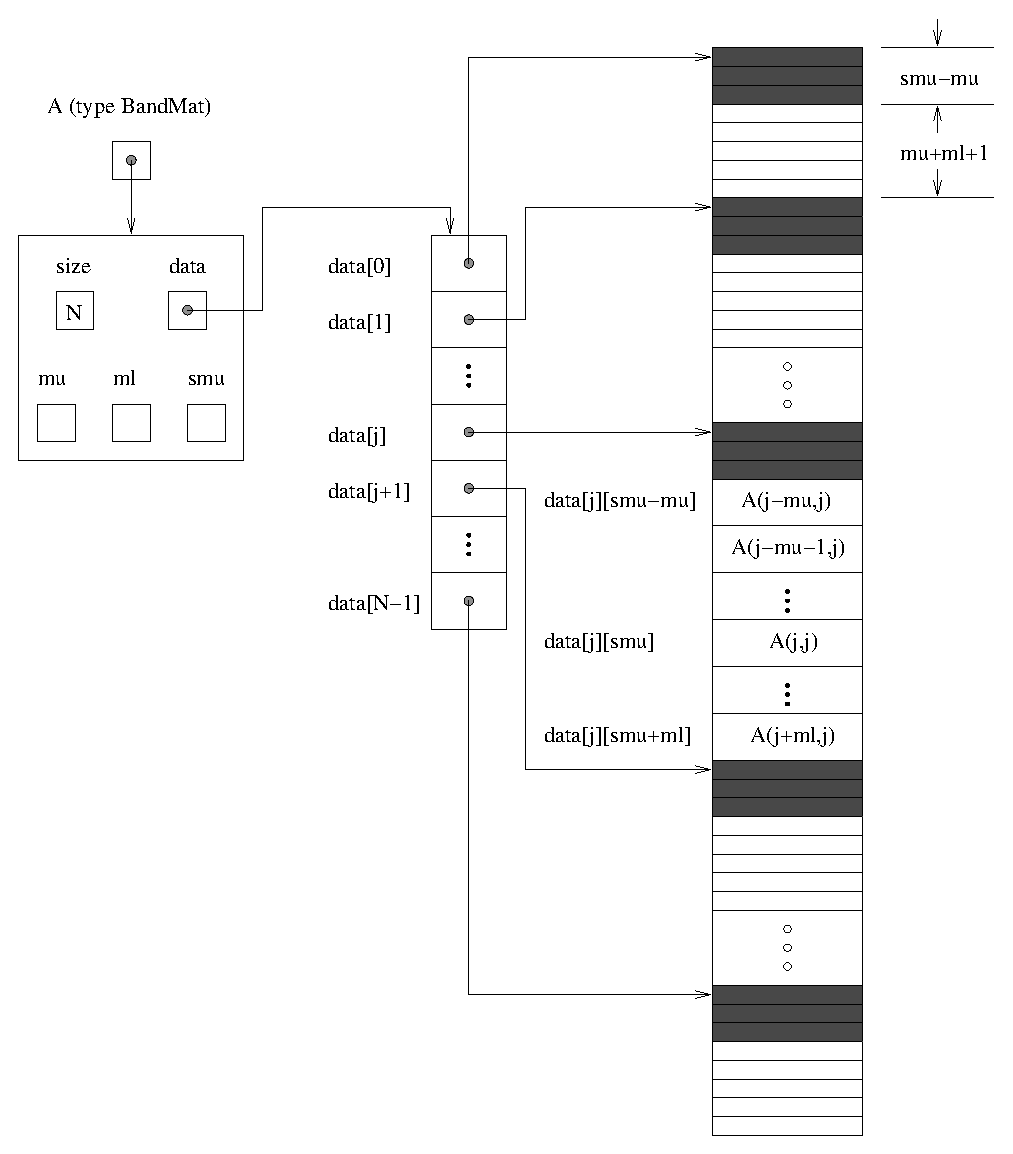
\includegraphics[width=4.5 in]{bandmat}}
\caption[Diagram of the storage for a {\sunmatband} object]
  {Diagram of the storage for the {\sunmatband} module. Here \id{A} is an
  $\id{N} \times \id{N}$ band matrix with upper and lower half-bandwidths \id{mu}
  and \id{ml}, respectively. The rows and columns of \id{A} are
  numbered from $0$ to $\id{N}-1$ and the ($i,j$)-th element of \id{A} is
  denoted \id{A(i,j)}. The greyed out areas of the underlying
  component storage are used by the associated {\sunlinsolband}
  linear solver.}\label{f:sunbandmat}
\end{figure}

\noindent The header file to include when using this module
is \id{sunmatrix/sunmatrix\_band.h}. The {\sunmatband} module
is accessible from all {\sundials} solvers \textit{without}
linking to the \newline
\id{libsundials\_sunmatrixband} module library.


% ====================================================================
\subsection{SUNMatrix\_Band accessor macros}
\label{ss:sunmat_band_macros}
% ====================================================================

The following macros are provided to access the
content of a {\sunmatband} matrix. The prefix \id{SM\_} in the names
denotes that these macros are for \emph{SUNMatrix} implementations,
and the suffix \id{\_B} denotes that these are specific to
the \emph{banded} version.
%%
\begin{itemize}

\item \ID{SM\_CONTENT\_B}

  This routine gives access to the contents of the
  banded \id{SUNMatrix}.

  The assignment \id{A\_cont} $=$ \id{SM\_CONTENT\_B(A)} sets
  \id{A\_cont} to be a pointer to the banded \id{SUNMatrix} content
  structure.

  Implementation:

  \verb|#define SM_CONTENT_B(A)     ( (SUNMatrixContent_Band)(A->content) )|

\item \ID{SM\_ROWS\_B}, \ID{SM\_COLUMNS\_B}, \ID{SM\_UBAND\_B}, \ID{SM\_LBAND\_B}, \ID{SM\_SUBAND\_B}, \ID{SM\_LDIM\_B}, and \ID{SM\_LDATA\_B}

  These macros give individual access to various lengths relevant to the
  content of a banded \id{SUNMatrix}.

  These may be used either to retrieve or to set these values.  For
  example, the assignment \id{A\_rows = SM\_ROWS\_B(A)} sets \id{A\_rows} to be
  the number of rows in the matrix \id{A}.  Similarly, the
  assignment \id{SM\_COLUMNS\_B(A) = A\_cols} sets the number of
  columns in \id{A} to equal \id{A\_cols}.

  Implementation:

  \verb|#define SM_ROWS_B(A)        ( SM_CONTENT_B(A)->M )|

  \verb|#define SM_COLUMNS_B(A)     ( SM_CONTENT_B(A)->N )|

  \verb|#define SM_UBAND_B(A)       ( SM_CONTENT_B(A)->mu )|

  \verb|#define SM_LBAND_B(A)       ( SM_CONTENT_B(A)->ml )|

  \verb|#define SM_SUBAND_B(A)      ( SM_CONTENT_B(A)->s_mu )|

  \verb|#define SM_LDIM_B(A)        ( SM_CONTENT_B(A)->ldim )|

  \verb|#define SM_LDATA_B(A)       ( SM_CONTENT_B(A)->ldata )|

\item \ID{SM\_DATA\_B} and \ID{SM\_COLS\_B}

  These macros give access to the \id{data} and \id{cols} pointers for
  the matrix entries.

  The assignment \id{A\_data = SM\_DATA\_B(A)} sets \id{A\_data} to be
  a pointer to the first component of the data array for the
  banded \id{SUNMatrix} \id{A}.  The assignment \id{SM\_DATA\_B(A) =
  A\_data} sets the data array of \id{A} to be \id{A\_data} by storing
  the pointer \id{A\_data}.

  Similarly, the assignment \id{A\_cols = SM\_COLS\_B(A)} sets \id{A\_cols} to be
  a pointer to the array of column pointers for the banded \id{SUNMatrix} \id{A}.
  The assignment \id{SM\_COLS\_B(A) = A\_cols} sets the column pointer
  array of \id{A} to be \id{A\_cols} by storing the pointer \id{A\_cols}.

  Implementation:

  \verb|#define SM_DATA_B(A)        ( SM_CONTENT_B(A)->data )|

  \verb|#define SM_COLS_B(A)        ( SM_CONTENT_B(A)->cols )|


\item \ID{SM\_COLUMN\_B}, \ID{SM\_COLUMN\_ELEMENT\_B}, and \ID{SM\_ELEMENT\_B}

  These macros give access to the individual columns and entries of
  the data array of a banded \id{SUNMatrix}.

  The assignments \id{SM\_ELEMENT\_B(A,i,j) = a\_ij} and \id{a\_ij =
  SM\_ELEMENT\_B(A,i,j)} reference the (\id{i},\id{j})-th element of the
  $\id{N} \times \id{N}$ band matrix \id{A}, where $0 \le \id{i}, \id{j} \le \id{N}-1$.
  The location (\id{i},\id{j}) should further satisfy
  \id{j}$-$\id{mu} $\le$ \id{i} $\le$ \id{j}$+$\id{ml}.

  The assignment \id{col\_j = SM\_COLUMN\_B(A,j)} sets \id{col\_j} to be
  a pointer to the diagonal element of the \id{j}-th column of the
  $\id{N} \times \id{N}$ band matrix \id{A}, $0 \le \id{j} \le \id{N}-1$.
  The type of the expression \id{SM\_COLUMN\_B(A,j)} is \id{realtype *}.
  The pointer returned by the call \id{SM\_COLUMN\_B(A,j)} can be treated as
  an array which is indexed from $-$\id{mu} to \id{ml}.

  The assignments \id{SM\_COLUMN\_ELEMENT\_B(col\_j,i,j) = a\_ij} and\\
  \id{a\_ij = SM\_COLUMN\_ELEMENT\_B(col\_j,i,j)} reference the
  (\id{i},\id{j})-th entry of the band matrix \id{A} when used in
  conjunction with \id{SM\_COLUMN\_B} to reference the \id{j}-th column
  through \id{col\_j}. The index (\id{i},\id{j}) should satisfy
  \id{j}$-$\id{mu} $\le$ \id{i} $\le$ \id{j}$+$\id{ml}.

  Implementation:

  \verb|#define SM_COLUMN_B(A,j)    ( ((SM_CONTENT_B(A)->cols)[j])+SM_SUBAND_B(A) )|

  \verb|#define SM_COLUMN_ELEMENT_B(col_j,i,j) (col_j[(i)-(j)])|

  \verb|#define SM_ELEMENT_B(A,i,j)|

  \hspace{1in} \verb|( (SM_CONTENT_B(A)->cols)[j][(i)-(j)+SM_SUBAND_B(A)] )|

\end{itemize}


% ====================================================================
\subsection{SUNMatrix\_Band functions}
\label{ss:sunmat_band_functions}
% ====================================================================

The {\sunmatband} module defines banded implementations of all matrix
operations listed in Table \ref{t:sunmatops}. Their names are obtained
from those in Table \ref{t:sunmatops} by appending the
suffix \id{\_Band} (e.g. \id{SUNMatCopy\_Band}).
All the standard matrix operations listed in \ref{t:sunmatops} with the suffix
\id{\_Band} appended are callable via the {\F} 2003 interface by prepending an
`F' (e.g. \id{FSUNMatCopy\_Band}).

The module {\sunmatband} provides the following additional user-callable routines:
%%--------------------------------------
\sunmodfunf{SUNBandMatrix}
{
  This constructor function creates and allocates memory for a banded \id{SUNMatrix}.
  Its arguments are the matrix size, \id{N}, and the upper and lower
  half-bandwidths of the matrix, \id{mu} and \id{ml}.  The stored
  upper bandwidth is set to \id{mu+ml} to accommodate subsequent
  factorization in the {\sunlinsolband} and {\sunlinsollapband} modules.
}
{
  SUNMatrix SUNBandMatrix(sunindextype N, sunindextype mu,
  sunindextype ml)
}
%%--------------------------------------
\sunmodfun{SUNBandMatrixStorage}
{
  This constructor function creates and allocates memory for a banded \id{SUNMatrix}.
  Its arguments are the matrix size, \id{N}, the upper and lower
  half-bandwidths of the matrix, \id{mu} and \id{ml}, and the stored
  upper bandwidth, \id{smu}.  When creating a band \id{SUNMatrix},
  this value should be
  \begin{itemize}
  \item at least min(\id{N}-1,\id{mu}+\id{ml}) if the matrix will be
    used by the {\sunlinsolband} module;
  \item exactly equal to \id{mu}+\id{ml} if the matrix will be used by
    the {\sunlinsollapband} module;
  \item at least \id{mu} if used in some other manner.
  \end{itemize}
  \emph{Note: it is strongly recommended that users call the default
    constructor, \id{SUNBandMatrix}, in all standard use cases.  This
    advanced constructor is used internally within {\sundials}
    solvers, and is provided to users who require banded matrices for
    non-default purposes.}
}
{
  SUNMatrix SUNBandMatrixStorage(sunindextype N, sunindextype mu,
  sunindextype ml, sunindextype smu)
}
%%--------------------------------------
\sunmodfun{SUNBandMatrix\_Print}
{
  This function prints the content of a banded \id{SUNMatrix} to the
  output stream specified by \id{outfile}.  Note: \id{stdout}
  or \id{stderr} may be used as arguments for \id{outfile} to print
  directly to standard output or standard error, respectively.
}
{
  void SUNBandMatrix\_Print(SUNMatrix A, FILE* outfile)
}
%%--------------------------------------
\sunmodfunf{SUNBandMatrix\_Rows}
{
  This function returns the number of rows in the banded \id{SUNMatrix}.
}
{
  sunindextype SUNBandMatrix\_Rows(SUNMatrix A)
}
%%--------------------------------------
\sunmodfunf{SUNBandMatrix\_Columns}
{
  This function returns the number of columns in the banded \id{SUNMatrix}.
}
{
  sunindextype SUNBandMatrix\_Columns(SUNMatrix A)
}
%%--------------------------------------
\sunmodfunf{SUNBandMatrix\_LowerBandwidth}
{
  This function returns the lower half-bandwidth of the banded \id{SUNMatrix}.
}
{
  sunindextype SUNBandMatrix\_LowerBandwidth(SUNMatrix A)
}
%%--------------------------------------
\sunmodfunf{SUNBandMatrix\_UpperBandwidth}
{
  This function returns the upper half-bandwidth of the banded \id{SUNMatrix}.
}
{
  sunindextype SUNBandMatrix\_UpperBandwidth(SUNMatrix A)
}
%%--------------------------------------
\sunmodfunf{SUNBandMatrix\_StoredUpperBandwidth}
{
  This function returns the stored upper half-bandwidth of the banded \id{SUNMatrix}.
}
{
  sunindextype SUNBandMatrix\_StoredUpperBandwidth(SUNMatrix A)
}
%%--------------------------------------
\sunmodfunf{SUNBandMatrix\_LDim}
{
  This function returns the length of the leading dimension of the banded \id{SUNMatrix}.
}
{
  sunindextype SUNBandMatrix\_LDim(SUNMatrix A)
}
%%--------------------------------------
\sunmodfunf{SUNBandMatrix\_Data}
{
  This function returns a pointer to the data array for the banded \id{SUNMatrix}.
}
{
  realtype* SUNBandMatrix\_Data(SUNMatrix A)
}
%%--------------------------------------
\sunmodfun{SUNBandMatrix\_Cols}
{
  This function returns a pointer to the cols array for the banded \id{SUNMatrix}.
}
{
  realtype** SUNBandMatrix\_Cols(SUNMatrix A)
}
%%--------------------------------------
\sunmodfunf{SUNBandMatrix\_Column}
{
  This function returns a pointer to the diagonal entry of the j-th
  column of the banded \id{SUNMatrix}.  The resulting pointer should
  be indexed over the range $-$\id{mu} to \id{ml}.
}
{
  realtype* SUNBandMatrix\_Column(SUNMatrix A, sunindextype j)
}
%%
%%------------------------------------
%%
\paragraph{\bf Notes}

\begin{itemize}

\item
  When looping over the components of a banded \id{SUNMatrix} \id{A},
  the most efficient approaches are to:
  \begin{itemize}
    \item First obtain the component array via \id{A\_data = SM\_DATA\_B(A)} or\\
    \id{A\_data = SUNBandMatrix\_Data(A)} and then
    access \id{A\_data[i]} within the loop.

    \item First obtain the array of column pointers via \id{A\_cols = SM\_COLS\_B(A)} or\\
    \id{A\_cols = SUNBandMatrix\_Cols(A)}, and then
    access \id{A\_cols[j][i]} within the loop.

    \item Within a loop over the columns, access the column pointer via\\
    \id{A\_colj = SUNBandMatrix\_Column(A,j)} and then to access the
    entries within that column using \id{SM\_COLUMN\_ELEMENT\_B(A\_colj,i,j)}.
  \end{itemize}
  All three of these are more efficient than
  using \id{SM\_ELEMENT\_B(A,i,j)} within a double loop.

\item
  {\warn} Within the \id{SUNMatMatvec\_Band} routine, internal
  consistency checks are performed to ensure that the matrix is called
  with consistent {\nvector} implementations.  These are currently
  limited to: {\nvecs}, {\nvecopenmp}, and {\nvecpthreads}.  As additional
  compatible vector implementations are added to {\sundials}, these
  will be included within this compatibility check.

\end{itemize}


% ====================================================================
\subsection{SUNMatrix\_Band Fortran interfaces}
\label{ss:sunmat_band_fortran}
% ====================================================================

The {\sunmatband} module provides a {\F} 2003 module as well as {\F} 77
style interface functions for use from {\F} applications.

\subsubsection*{FORTRAN 2003 interface module}
The \ID{fsunmatrix\_band\_mod} {\F} module defines interfaces to most
{\sunmatband} {\CC} functions using the intrinsic \id{iso\_c\_binding}
module which provides a standardized mechanism for interoperating with {\CC}. As
noted in the {\CC} function descriptions above, the interface functions are
named after the corresponding {\CC} function, but with a leading `F'. For
example, the function \id{SUNBandMatrix} is interfaced as
\id{FSUNBandMatrix}.

The {\F} 2003 {\sunmatband} interface module can be accessed with the \id{use}
statement, i.e. \id{use fsunmatrix\_band\_mod}, and linking to the library
\id{libsundials\_fsunmatrixband\_mod}.{\em lib} in addition to the {\CC} library.
For details on where the library and module file
\id{fsunmatrix\_band\_mod.mod} are installed see Appendix \ref{c:install}.
We note that the module is accessible from the {\F} 2003 {\sundials} integrators
\textit{without} separately linking to the
\id{libsundials\_fsunmatrixband\_mod} library.

\subsubsection*{FORTRAN 77 interface functions}
For solvers that include a {\F} interface module, the {\sunmatband}
module also includes the {\F}-callable
function \id{FSUNBandMatInit(code, N, mu, ml, ier)} to initialize
this {\sunmatband} module for a given {\sundials} solver.
Here \id{code} is an integer input solver id (1 for {\cvode}, 2 for {\ida}, 3
for {\kinsol}, 4 for {\arkode}); \id{N}, \id{mu}, and \id{ml}
are the corresponding band matrix construction arguments (declared
to match C type \id{long int}); and \id{ier} is an error return flag
equal to 0 for success and -1 for failure. Both \id{code} and \id{ier}
are declared to match C type \id{int}. Additionally, when using
{\arkode} with a non-identity mass matrix, the {\F}-callable
function \id{FSUNBandMassMatInit(N, mu, ml, ier)} initializes
this {\sunmatband} module for storing the mass matrix.


%---------------------------------------------------------------------------
\section{The SUNMatrix\_Dense implementation}\label{ss:sunmat_dense}
%% This is a shared SUNDIALS TEX file with a description of the
%% dense sunmatrix implementation
%%

The dense implementation of the {\sunmatrix} module provided with
{\sundials}, {\sunmatdense}, defines the {\em content} field
of \id{SUNMatrix} to be the following structure:
%%
\begin{verbatim} 
struct _SUNMatrixContent_Dense {
  sunindextype M;
  sunindextype N;
  realtype *data;
  sunindextype ldata;
  realtype **cols;
};
\end{verbatim}
%%
These entries of the \emph{content} field contain the following
information:
\begin{description}
  \item[M] - number of rows
  \item[N] - number of columns
  \item[data] - pointer to a contiguous block of \id{realtype} variables.
    The elements of the dense matrix are stored columnwise, i.e.~the
    (\id{i},\id{j})-th element of a dense {\sunmatrix} \id{A} 
    (with $0 \le$ \id{i} $<$ \id{M} and $ 0 \le$ \id{j} $<$ \id{N}) 
    may be accessed via \id{data[j*M+i]}.
  \item[ldata] - length of the data array ($=$ \id{M}$\cdot$\id{N}).
  \item[cols] - array of pointers. \id{cols[j]} points to the first
    element of the j-th column of the matrix in the array \id{data}.
    The (\id{i},\id{j})-th element of a dense {\sunmatrix} \id{A}
    (with $0 \le$ \id{i} $<$ \id{M} and $ 0 \le$ \id{j} $<$ \id{N}) 
    may be accessed via \id{cols[j][i]}.
\end{description}

\noindent The header file to be included when using this module 
is \id{sunmatrix/sunmatrix\_dense.h}. \\

\noindent The following eight macros are provided to access the
content of a {\sunmatdense} matrix. The prefix \id{SM\_} in the names
denotes that these macros are for \emph{SUNMatrix} implementations,
and the suffix \id{\_D} denotes that these are specific to
the \emph{dense} version.
%%
\begin{itemize}

\item \ID{SM\_CONTENT\_D}
    
  This routine gives access to the contents of the
  dense \id{SUNMatrix}.
  
  The assignment \id{A\_cont} $=$ \id{SM\_CONTENT\_D(A)} sets
  \id{A\_cont} to be a pointer to the dense \id{SUNMatrix} content  
  structure.                                             
                                                            
  Implementation: 
  
  \verb|#define SM_CONTENT_D(A)     ( (SUNMatrixContent_Dense)(A->content) )|
  
\item \ID{SM\_ROWS\_D}, \ID{SM\_COLUMNS\_D}, and \ID{SM\_LDATA\_D}

  These macros give individual access various lengths relevant to the
  content of a dense \id{SUNMatrix}.                        
                                                               
  These may be used either to retrieve or to set these values.  For
  example, the assignment \id{A\_rows = SM\_ROWS\_D(A)} sets \id{A\_rows} to be
  the number of rows in the matrix \id{A}.  Similarly, the
  assignment \id{SM\_COLUMNS\_D(A) = A\_cols} sets the number of
  columns in \id{A} to equal \id{A\_cols}.
  
  Implementation: 

  \verb|#define SM_ROWS_D(A)        ( SM_CONTENT_D(A)->M )|

  \verb|#define SM_COLUMNS_D(A)     ( SM_CONTENT_D(A)->N )|

  \verb|#define SM_LDATA_D(A)       ( SM_CONTENT_D(A)->ldata )|

\item \ID{SM\_DATA\_D} and \ID{SM\_COLS\_D}
                                                            
  These macros give access to the \id{data} and \id{cols} pointers for
  the matrix entries.

  The assignment \id{A\_data = SM\_DATA\_D(A)} sets \id{A\_data} to be     
  a pointer to the first component of the data array for the dense
  \id{SUNMatrix} \id{A}.  The assignment \id{SM\_DATA\_D(A) = A\_data}
  sets the data array of \id{A} to be \id{A\_data} by storing the
  pointer \id{A\_data}.
  
  Similarlly, the assignment \id{A\_cols = SM\_COLS\_D(A)} sets \id{A\_cols} to be     
  a pointer to the array of column pointers for the dense \id{SUNMatrix} \id{A}. 
  The assignment \id{SM\_COLS\_D(A) = A\_cols} sets the column pointer
  array of \id{A} to be \id{A\_cols} by storing the pointer \id{A\_cols}.                   
  
  Implementation:

  \verb|#define SM_DATA_D(A)        ( SM_CONTENT_D(A)->data )|

  \verb|#define SM_COLS_D(A)        ( SM_CONTENT_D(A)->cols )|


\item \ID{SM\_COLUMN\_D} and \ID{SM\_ELEMENT\_D}
                                                            
  These macros gives access to the individual columns and entries of
  the data array of a dense \id{SUNMatrix}.

  The assignment \id{col\_j = SM\_COLUMN\_D(A,j)} sets \id{col\_j} to be
  a pointer to the first entry of the \id{j}-th column of the $M \times N$
  dense matrix \id{A}, $0 \le$ \id{j} $< N$.  The type of the
  expression \id{SM\_COLUMN\_D(A,j)} is \id{realtype *}.  The pointer
  returned by the call \id{SM\_COLUMN\_D(A,j)} can be treated as  
  an array which is indexed from $0$ to $M-1$.

  The assignments \id{SM\_ELEMENT\_D(A,i,j) = a\_ij} and \id{a\_ij =
  SM\_ELEMENT\_D(A,i,j)} reference the (\id{i},\id{j})-th element of the
  $M \times N$ dense matrix \id{A}, where $0 \le$ \id{i} $< M$ and
  $0\le $ \id{j} $< N$.

  Implementation:

  \verb|#define SM_COLUMN_D(A,j)    ( (SM_CONTENT_D(A)->cols)[j] )|

  \verb|#define SM_ELEMENT_D(A,i,j) ( (SM_CONTENT_D(A)->cols)[j][i] )|

\end{itemize}
%%
%%----------------------------------------------
%%
The {\sunmatdense} module defines dense implementations of all matrix
operations listed in Table \ref{t:sunmatops}. Their names are obtained
from those in Table \ref{t:sunmatops} by appending the
suffix \id{\_Dense} (e.g. \id{SUNMatCopy\_Dense}). 
The module {\sunmatdense} provides the following additional
user-callable routines: 
%%
\begin{itemize}

%%--------------------------------------

\item \ID{SUNDenseMatrix}

  This function creates and allocates memory for a dense \id{SUNMatrix}.
  Its arguments are the number of rows, \id{M}, and columns, \id{N}, for
  the dense matrix.

  \verb|SUNMatrix SUNDenseMatrix(sunindextype M, sunindextype N);|

%%--------------------------------------

\item \ID{SUNDenseMatrix\_Print}

  This function prints the content of a dense \id{SUNMatrix} to the
  output stream specified by \id{outfile}.  Note: \id{stdout}
  or \id{stderr} may be used as arguments for \id{outfile} to print
  directly to standard output or standard error, respectively.
 
  \verb|void SUNDenseMatrix_Print(SUNMatrix A, FILE* outfile);|

%%--------------------------------------

\item \ID{SUNDenseMatrix\_Rows}

  This function returns the number of rows in the dense \id{SUNMatrix}.
 
  \verb|sunindextype SUNDenseMatrix_Rows(SUNMatrix A);|

%%--------------------------------------

\item \ID{SUNDenseMatrix\_Columns}

  This function returns the number of columns in the dense \id{SUNMatrix}.
 
  \verb|sunindextype SUNDenseMatrix_Columns(SUNMatrix A);|

%%--------------------------------------

\item \ID{SUNDenseMatrix\_LData}

  This function returns the length of the data array for the dense \id{SUNMatrix}.
 
  \verb|sunindextype SUNDenseMatrix_LData(SUNMatrix A);|

%%--------------------------------------

\item \ID{SUNDenseMatrix\_Data}

  This function returns a pointer to the data array for the dense \id{SUNMatrix}.
 
  \verb|realtype* SUNDenseMatrix_Data(SUNMatrix A);|

%%--------------------------------------

\item \ID{SUNDenseMatrix\_Cols}

  This function returns a pointer to the cols array for the dense \id{SUNMatrix}.
 
  \verb|realtype** SUNDenseMatrix_Cols(SUNMatrix A);|

%%--------------------------------------

\item \ID{SUNDenseMatrix\_Column}

  This function returns a pointer to the first entry of the jth
  column of the dense \id{SUNMatrix}.  The resulting pointer should
  be indexed over the range $0$ to $M-1$.
 
  \verb|realtype* SUNDenseMatrix_Column(SUNMatrix A, sunindextype j);|

\end{itemize}
%%
%%------------------------------------
%%
\paragraph{\bf Notes}                                                      
           
\begin{itemize}
                                        
\item
  When looping over the components of a dense \id{SUNMatrix} \id{A},
  the most efficient approaches are to:
  \begin{itemize}
    \item First obtain the component array via \id{A\_data = SM\_DATA\_D(A)} or\\
    \id{A\_data = SUNDenseMatrix\_Data(A)} and then
    access \id{A\_data[i]} within the loop.
  
    \item First obtain the array of column pointers via \id{A\_cols = SM\_COLS\_D(A)} or\\
    \id{A\_cols = SUNDenseMatrix\_Cols(A)}, and then
    access \id{A\_cols[j][i]} within the loop. 
  
    \item Within a loop over the columns, access the column pointer via\\
    \id{A\_colj = SUNDenseMatrix\_Column(A,j)} and then to access the
    entries within that column using \id{A\_colj[i]} within the loop.
  \end{itemize}
  All three of these are more efficient than
  using \id{SM\_ELEMENT\_D(A,i,j)} within a double loop.

\item
  {\warn} Within the \id{SUNMatMatvec\_Dense} routine, internal
  consistency checks are performed to ensure that the matrix is called
  with consistent {\nvector} implementations.  These are currently
  limited to: {\nvecs}, {\nvecopenmp} and {\nvecpthreads}.  As additional
  compatible vector implementations are added to {\sundials}, these
  will be included within this compatibility check.

\end{itemize}

For solvers that include a Fortran interface module, the {\sunmatdense}
module also includes the Fortran-callable
function \id{FSUNDenseMatInit(code, M, N, ier)} to initialize
this {\sunmatdense} module for a given {\sundials} solver.
Here \id{code} is an input solver id (1 for {\cvode}, 2 for {\ida}, 3
for {\kinsol}, 4 for {\arkode}); \id{M} and \id{N} are the
corresponding dense matrix construction arguments (declared so as to
match C type \id{long int}); and \id{ier} is an error return flag 
equal 0 for success and -1 for failure (declared so as to match C type
\id{int}). Additionally, when using {\arkode} with non-identity mass
matrix, the Fortran-callable function \id{FSUNDenseMassMatInit(M, N, ier)} 
initializes this {\sunmatdense} module for storing the mass matrix.


%---------------------------------------------------------------------------
\section{The SUNMatrix\_Diagonal implementation}\label{ss:sunmat_diag}
%% This is a shared SUNDIALS TEX file with a description of the
%% diagonal sunmatrix implementation
%%

The diagonal implementation of the {\sunmatrix} module provided with
{\sundials}, {\sunmatdiag}, defines the {\em content} field
of \id{SUNMatrix} to be the following structure:
%%
\begin{verbatim} 
struct _SUNMatrixContent_Diagonal {
  N_Vector d;
};
\end{verbatim}
%%
The entry of the \emph{content} field contain the following
information:
\begin{description}
  \item[d] - generic {\nvector} object containing the diagonal of the
  {\sunmatrix}.
\end{description}

\noindent The header file to be included when using this module 
is \id{sunmatrix/sunmatrix\_diagonal.h}. \\

\noindent The following two macros are provided to access the
content of a {\sunmatdiag} matrix. The prefix \id{SM\_} in the names
denotes that these macros are for \emph{SUNMatrix} implementations,
and the suffix \id{\_DIAG} denotes that these are specific to
the \emph{diagonal} version.
%%
\begin{itemize}

\item \ID{SM\_CONTENT\_DIAG}
    
  This routine gives access to the contents of the
  diagonal \id{SUNMatrix}.
  
  The assignment \id{A\_cont} $=$ \id{SM\_CONTENT\_DIAG(A)} sets
  \id{A\_cont} to be a pointer to the diagonal \id{SUNMatrix} content
  structure.                                             
                                                            
  Implementation: 
  
  \verb|#define SM_CONTENT_DIAG(A)  ( (SUNMatrixContent_Diagonal)(A->content) )|
  
\item \ID{SM\_DATA\_DIAG}
                                                            
  This macro gives access to the {\nvector} \id{d} that defines the
  diagonal matrix.

  The assignment \id{A\_data = SM\_DATA\_DIAG(A)} sets \id{A\_data} to be     
  the {\nvector} storing the matrix diagonal.  The
  assignment \id{SM\_DATA\_DIAG(A) = A\_data} sets the {\nvector}
  matrix diagonal to \id{A\_data}.
  
  Implementation:

  \verb|#define SM_DATA_DIAG(A)     ( SM_CONTENT_DIAG(A)->d )|

\end{itemize}
%%
%%----------------------------------------------
%%
The {\sunmatdiag} module defines diagonal implementations of all
matrix operations listed in Table \ref{t:sunmatops}. Their names are
obtained from those in Table \ref{t:sunmatops} by appending the
suffix \id{\_Diagonal} (e.g. \id{SUNMatCopy\_Diagonal}). 
The module {\sunmatdiag} provides the following additional
user-callable routines: 
%%
\begin{itemize}

%%--------------------------------------

\item \ID{SUNDiagonalMatrix}

  This function creates and allocates memory for a diagonal \id{SUNMatrix}.
  Its argument is a template {\nvector} object.

  \verb|SUNMatrix SUNDiagonalMatrix(N_Vector tmpl);|

%%--------------------------------------

\item \ID{SUNDiagonalMatrix\_Diag}

  This function returns the {\nvector} containing the diagonal of
  the \id{SUNMatrix}. 
 
  \verb|N_Vector SUNDiagonalMatrix_Diag(SUNMatrix A);|

\end{itemize}
%%
%%------------------------------------
%%
\paragraph{\bf Notes}                                                      
           
\begin{itemize}
                                        
\item
  To access the components of a diagonal \id{SUNMatrix} \id{A}, you
  must first retrieve the {\nvector} containing the matrix diagonal
  via \id{A\_data = SM\_DATA\_DIAG(A)} or\\
  \id{A\_data = SUNDiagonalMatrix\_Diag(A)}, and then access the
  entries of the {\nvector} using whichever macros or functions are
  appropriate for that {\nvector} implementation.

\item
  Within the \id{SUNMatMatvec\_Diagonal} routine, internal consistency
  checks are performed to ensure that the matrix is called with
  consistent {\nvector} implementations.  This consistency check
  merely ensures that the matrix diagonal, as well as the input 
  {\nvector} objects \id{x} and \id{y} all have
  identical \id{N\_Vector\_ID}.  As such, this routine may be used
  with any {\sundials}-supplied or user-supplied {\nvector}
  implementation. 

\end{itemize}

For solvers that include a Fortran interface module, the {\sunmatdiag}
module also includes the Fortran-callable
function \id{FSUNDiagonalMatInit(code, ier)} to initialize
this {\sunmatdiag} module for a given {\sundials} solver.
Here \id{code} is an input solver id (1 for {\cvode}, 2 for {\ida}, 3
for {\kinsol}, 4 for {\arkode}); and \id{ier} is an error return flag 
equal 0 for success and -1 for failure (declared so as to match C type
\id{int}).  This routine must be called \emph{after} a corresponding
{\nvector} has been initialized by a call to \id{FNVInit*}.
Additionally, when using {\arkode} with non-identity mass matrix, the
Fortran-callable function \id{FSUNDiagonalMassMatInit(ier)}  
initializes this {\sunmatdiag} module for storing the mass matrix.


%---------------------------------------------------------------------------
\section{The SUNMatrix\_Sparse implementation}\label{ss:sunmat_sparse}
%% This is a shared SUNDIALS TEX file with a description of the
%% sparse sunmatrix implementation
%%
\section{The SUNMatrix\_Sparse implementation}\label{ss:sunmat_sparse}

The sparse implementation of the {\sunmatrix} module provided with
{\sundials}, {\sunmatsparse}, is designed to work with either
\emph{compressed-sparse-column} (CSC) or \emph{compressed-sparse-row}
(CSR) sparse matrix formats.  To this end, it defines the {\em
content} field of \id{SUNMatrix} to be the following structure:
%%
\begin{verbatim} 
struct _SUNMatrixContent_Sparse {
  sunindextype M;
  sunindextype N;
  sunindextype NNZ;
  sunindextype NP;
  realtype *data;
  int sparsetype;
  sunindextype *indexvals;
  sunindextype *indexptrs;
  /* CSC indices */
  sunindextype **rowvals;
  sunindextype **colptrs;
  /* CSR indices */
  sunindextype **colvals;
  sunindextype **rowptrs;
};
\end{verbatim}
%%
A diagram of the underlying data representation for a
CSC matrix is shown in Figure \ref{f:sparsemat} (the CSR format is
similar).  A more complete description of the parts of
this \emph{content} field is given below: 
\begin{args}[sparsetype]
  \item[M]  - number of rows
  \item[N]  - number of columns
  \item[NNZ]  - maximum number of nonzero entries in the matrix
    (allocated length of \id{data} and \id{indexvals} arrays)
  \item[NP]  - number of index pointers (e.g. number of column pointers for 
    CSC matrix). For CSC matrices $\id{NP}=\id{N}$, and for CSR
    matrices $\id{NP}=\id{M}$. This value is set automatically based
    the input for \verb|sparsetype|.
  \item[data]  - pointer to a contiguous block of \id{realtype}
    variables (of length \id{NNZ}), containing the values of the
    nonzero entries in the matrix
  \item[sparsetype]  - type of the sparse matrix (\id{CSC\_MAT} or \id{CSR\_MAT})
  \item[indexvals] - pointer to a contiguous block of \id{int} variables
    (of length \id{NNZ}), containing the row indices (if CSC) or column
   indices (if CSR) of each nonzero matrix entry held in \id{data}
  \item[indexptrs]  - pointer to a contiguous block of \id{int}
    variables (of length \id{NP+1}). For CSC matrices each 
    entry provides the index of the first column entry into the 
    \id{data} and \id{indexvals} arrays, e.g. if \id{indexptr[3]=7}, then 
    the first nonzero entry in the fourth column of the matrix is 
    located in \id{data[7]}, and is located in row \id{indexvals[7]} of the 
    matrix.  The last entry contains the total number of nonzero values in 
    the matrix and hence points one past the end of the active data in the 
    \id{data} and \id{indexvals} arrays. For CSR matrices, each entry provides 
    the index of the first row entry into the \id{data} and \id{indexvals} 
    arrays.
\end{args}
\noindent The following pointers are added to the \id{SlsMat} type for
  user convenience, to provide a more intuitive interface to the CSC
  and CSR sparse matrix data structures. They are set automatically
  when creating a sparse {\sunmatrix}, based on the sparse matrix storage
  type.  
\begin{args}[colptrs]
  \item[rowvals] - pointer to \verb|indexvals| when \id{sparsetype} is \id{CSC\_MAT},
    otherwise set to \verb|NULL|.
  \item[colptrs] - pointer to \verb|indexptrs| when \id{sparsetype} is \id{CSC\_MAT},
    otherwise set to \verb|NULL|.
  \item[colvals] - pointer to \verb|indexvals| when \id{sparsetype} is \id{CSR\_MAT},
    otherwise set to \verb|NULL|.
  \item[rowptrs] - pointer to \verb|indexptrs| when \id{sparsetype} is \id{CSR\_MAT},
    otherwise set to \verb|NULL|.
\end{args}
For example, the $5\times 4$ CSC matrix
\[
  \left[\begin{array}{cccc} 
     0 & 3 & 1 & 0\\
     3 & 0 & 0 & 2\\
     0 & 7 & 0 & 0\\
     1 & 0 & 0 & 9\\
     0 & 0 & 0 & 5
  \end{array}\right]
\]
could be stored in this structure as either
\begin{verbatim}
  M = 5;
  N = 4;
  NNZ = 8;
  NP = N;
  data = {3.0, 1.0, 3.0, 7.0, 1.0, 2.0, 9.0, 5.0};
  sparsetype = CSC_MAT;
  indexvals = {1, 3, 0, 2, 0, 1, 3, 4};
  indexptrs = {0, 2, 4, 5, 8};
\end{verbatim}
or 
\begin{verbatim}
  M = 5;
  N = 4;
  NNZ = 10;
  NP = N;
  data = {3.0, 1.0, 3.0, 7.0, 1.0, 2.0, 9.0, 5.0, *, *};
  sparsetype = CSC_MAT;
  indexvals = {1, 3, 0, 2, 0, 1, 3, 4, *, *};
  indexptrs = {0, 2, 4, 5, 8};
\end{verbatim}
where the first has no unused space, and the second has additional
storage (the entries marked with \texttt{*} may contain any values).
Note in both cases that the final value in \id{indexptrs} is $8$,
indicating the total number of nonzero entries in the matrix.

Similarly, in CSR format, the same matrix could be stored as
\begin{verbatim}
  M = 5;
  N = 4;
  NNZ = 8;
  NP = M;
  data = {3.0, 1.0, 3.0, 2.0, 7.0, 1.0, 9.0, 5.0};
  sparsetype = CSR_MAT;
  indexvals = {1, 2, 0, 3, 1, 0, 3, 3};
  indexptrs = {0, 2, 4, 5, 7, 8};
\end{verbatim}

%%
%%--------------------------------------------
%%
\begin{figure}
\centerline{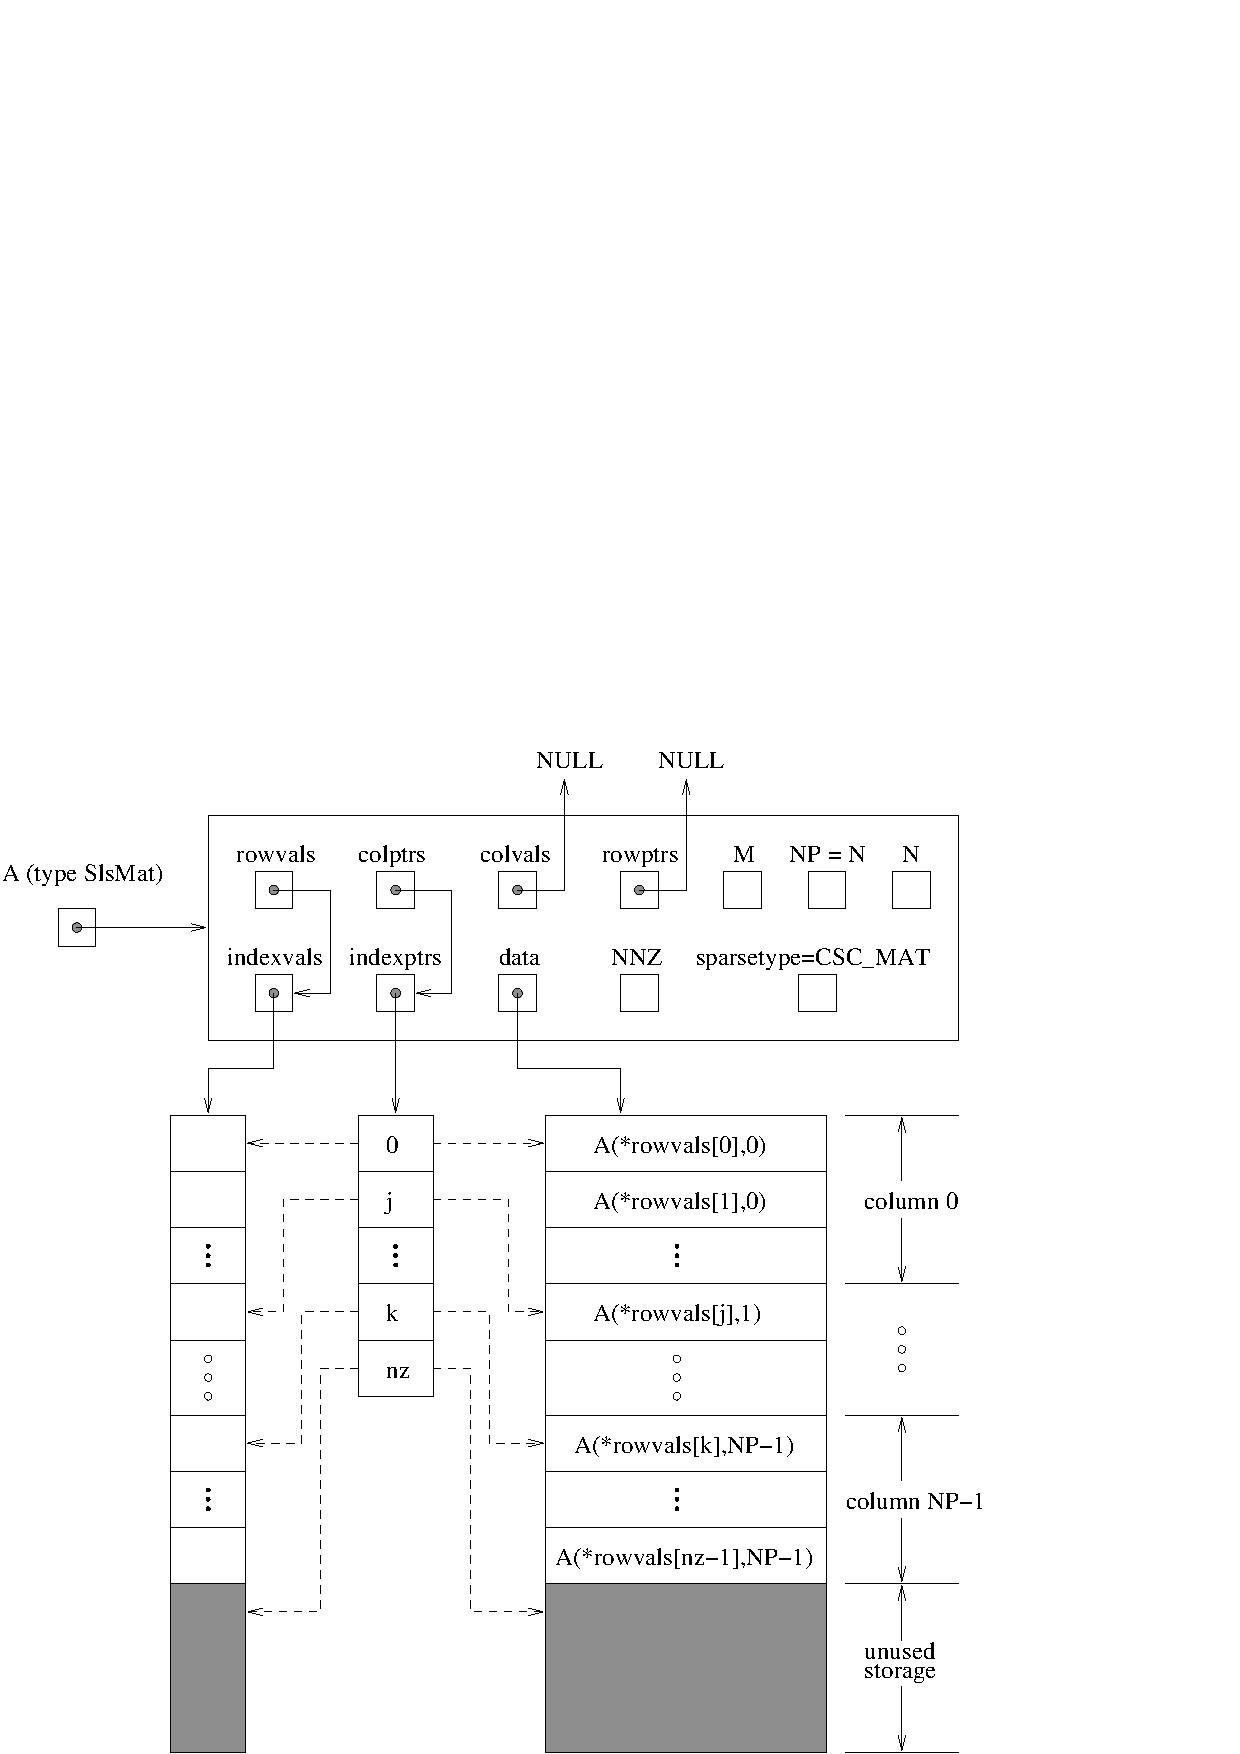
\includegraphics[width=4.5 in]{cscmat}}
\caption[Diagram of the storage for a compressed-sparse-column matrix] 
  {Diagram of the storage for a compressed-sparse-column
  matrix. Here \id{A} is an $\id{M} \times \id{N}$ sparse matrix with storage
  for up to \id{NNZ} nonzero entries (the allocated length of
  both \id{data} and \id{indexvals}).  The entries in \id{indexvals}
  may assume values from $0$ to $\id{M}-1$, corresponding to the row index
  (zero-based) of each nonzero value.  The entries in \id{data} contain
  the values of the nonzero entries, with the row $i$, column $j$
  entry of \id{A} (again, zero-based) denoted as \id{A(i,j)}.
  The \id{indexptrs} array contains $\id{N}+1$ entries; the first $\id{N}$
  denote the starting index of each column within the \id{indexvals}
  and \id{data} arrays, while the final entry points one past the
  final nonzero entry.  Here, although \id{NNZ} values are allocated,
  only \id{nz} are actually filled in; the greyed-out portions
  of \id{data} and \id{indexvals} indicate extra allocated
  space.}\label{f:sparsemat} 
\end{figure}

\noindent The header file to include when using this module 
is \id{sunmatrix/sunmatrix\_sparse.h}. The {\sunmatsparse} module
is accessible from all {\sundials} solvers \textit{without}
linking to the \\
\id{libsundials\_sunmatrixsparse} module library.


% ====================================================================
\subsection{SUNMatrix\_Sparse accessor macros}
\label{ss:sunmat_sparse_macros}
% ====================================================================

The following macros are provided to access the
content of a {\sunmatsparse} matrix. The prefix \id{SM\_} in the names
denotes that these macros are for \emph{SUNMatrix} implementations,
and the suffix \id{\_S} denotes that these are specific to
the \emph{sparse} version.
%%
\begin{itemize}

\item \ID{SM\_CONTENT\_S}
    
  This routine gives access to the contents of the
  sparse \id{SUNMatrix}.
  
  The assignment \id{A\_cont} $=$ \id{SM\_CONTENT\_S(A)} sets           
  \id{A\_cont} to be a pointer to the sparse \id{SUNMatrix} content  
  structure.                                             
                                                            
  Implementation: 
  
  \verb|#define SM_CONTENT_S(A)     ( (SUNMatrixContent_Sparse)(A->content) )|
  
\item \ID{SM\_ROWS\_S}, \ID{SM\_COLUMNS\_S}, \ID{SM\_NNZ\_S}, \ID{SM\_NP\_S}, and \ID{SM\_SPARSETYPE\_S}

  These macros give individual access to various lengths relevant to the
  content of a sparse \id{SUNMatrix}.
                                                               
  These may be used either to retrieve or to set these values.  For
  example, the assignment \id{A\_rows = SM\_ROWS\_S(A)} sets \id{A\_rows} to be
  the number of rows in the matrix \id{A}.  Similarly, the
  assignment \id{SM\_COLUMNS\_S(A) = A\_cols} sets the number of
  columns in \id{A} to equal \id{A\_cols}.
  
  Implementation: 
  
  \verb|#define SM_ROWS_S(A)        ( SM_CONTENT_S(A)->M )|

  \verb|#define SM_COLUMNS_S(A)     ( SM_CONTENT_S(A)->N )|

  \verb|#define SM_NNZ_S(A)         ( SM_CONTENT_S(A)->NNZ )|

  \verb|#define SM_NP_S(A)          ( SM_CONTENT_S(A)->NP )|

  \verb|#define SM_SPARSETYPE_S(A)  ( SM_CONTENT_S(A)->sparsetype )|


\item \ID{SM\_DATA\_S}, \ID{SM\_INDEXVALS\_S}, and \ID{SM\_INDEXPTRS\_S}
                                                            
  These macros give access to the \id{data} and index arrays for
  the matrix entries.

  The assignment \id{A\_data = SM\_DATA\_S(A)} sets \id{A\_data} to be     
  a pointer to the first component of the data array for the
  sparse \id{SUNMatrix} \id{A}.  The assignment \id{SM\_DATA\_S(A) =
  A\_data} sets the data array of \id{A} to be \id{A\_data} by storing
  the pointer \id{A\_data}. 
  
  Similarly, the assignment \id{A\_indexvals = SM\_INDEXVALS\_S(A)}
  sets \id{A\_indexvals} to be a pointer to the array of index values
  (i.e.~row indices for a CSC matrix, or column indices for a CSR
  matrix) for the sparse \id{SUNMatrix} \id{A}.  The
  assignment \id{A\_indexptrs = SM\_INDEXPTRS\_S(A)}
  sets \id{A\_indexptrs} to be a pointer to the array of index
  pointers (i.e.~the starting indices in the data/indexvals arrays for
  each row or column in CSR or CSC formats, respectively).
  
  Implementation:

  \verb|#define SM_DATA_S(A)        ( SM_CONTENT_S(A)->data )|

  \verb|#define SM_INDEXVALS_S(A)   ( SM_CONTENT_S(A)->indexvals )|

  \verb|#define SM_INDEXPTRS_S(A)   ( SM_CONTENT_S(A)->indexptrs )|

\end{itemize}


% ====================================================================
\subsection{SUNMatrix\_Sparse functions}
\label{ss:sunmat_sparse_functions}
% ====================================================================

The {\sunmatsparse} module defines sparse implementations of all matrix
operations listed in Section \ref{ss:sunmatrix_functions}. Their names are obtained
from those in Section \ref{ss:sunmatrix_functions} by appending the
suffix \id{\_Sparse} (e.g. \id{SUNMatCopy\_Sparse}). 
All the standard matrix operations listed in Section \ref{ss:sunmatrix_functions} with the suffix
\id{\_Sparse} appended are callable via the {\F} 2003 interface by prepending an
`F' (e.g. \id{FSUNMatCopy\_Sparse}).

The module {\sunmatsparse} provides the following additional
user-callable routines: 
%%--------------------------------------
\sunmodfunf{SUNSparseMatrix}
{
  This function creates and allocates memory for a sparse \id{SUNMatrix}.
  Its arguments are the number of rows and columns of the
  matrix, \id{M} and \id{N}, the maximum number of nonzeros to be
  stored in the matrix, \id{NNZ}, and a flag \id{sparsetype}
  indicating whether to use CSR or CSC format (valid arguments
  are \id{CSR\_MAT} or \id{CSC\_MAT}). 
}
{
  SUNMatrix SUNSparseMatrix(sunindextype M, sunindextype N,
  \newlinefill{SUNMatrix SUNSparseMatrix}
  sunindextype NNZ, int sparsetype)
}
%%--------------------------------------
\sunmodfunf{SUNSparseFromDenseMatrix}
{
  This function creates a new sparse matrix from an existing dense
  matrix by copying all values with magnitude larger than \id{droptol}
  into the sparse matrix structure.

  Requirements:
  \begin{itemize}
  \item \id{A} must have type \id{SUNMATRIX\_DENSE};
  \item \id{droptol} must be non-negative;
  \item \id{sparsetype} must be either \id{CSC\_MAT} or \id{CSR\_MAT}.
  \end{itemize}
  The function returns NULL if any requirements are violated, or if
  the matrix storage request cannot be satisfied. 
}
{
  SUNMatrix SUNSparseFromDenseMatrix(SUNMatrix A, realtype droptol,
  \newlinefill{SUNMatrix SUNSparseFromDenseMatrix}
  int sparsetype);
}
%%--------------------------------------
\sunmodfunf{SUNSparseFromBandMatrix}
{
  This function creates a new sparse matrix from an existing band
  matrix by copying all values with magnitude larger than \id{droptol}
  into the sparse matrix structure.

  Requirements:
  \begin{itemize}
  \item \id{A} must have type \id{SUNMATRIX\_BAND};
  \item \id{droptol} must be non-negative;
  \item \id{sparsetype} must be either \id{CSC\_MAT} or \id{CSR\_MAT}.
  \end{itemize}
  The function returns NULL if any requirements are violated, or if
  the matrix storage request cannot be satisfied. 
}
{
  SUNMatrix SUNSparseFromBandMatrix(SUNMatrix A, realtype droptol,
  \newlinefill{SUNMatrix SUNSparseFromBandMatrix}
  int sparsetype);
}
%%--------------------------------------
\sunmodfunf{SUNSparseMatrix\_Realloc}
{
  This function reallocates internal storage arrays in a sparse matrix
  so that the resulting sparse matrix has no wasted space (i.e.~the
  space allocated for nonzero entries equals the actual number of
  nonzeros, \id{indexptrs[NP]}). Returns 0 on success and 
  1 on failure (e.g.~if the input matrix is not sparse).
}
{
  int SUNSparseMatrix\_Realloc(SUNMatrix A)
}
%%--------------------------------------
\sunmodfunf{SUNSparseMatrix\_Reallocate}
{
  This function reallocates internal storage arrays in a sparse matrix
  so that the resulting sparse matrix has storage for a specified
  number of nonzeros. Returns 0 on success and 
  1 on failure (e.g.~if the input matrix is not sparse or if NNZ is
  negative). 
}
{
  int SUNSparseMatrix\_Reallocate(SUNMatrix A, sunindextype NNZ)
}
%%--------------------------------------
\sunmodfun{SUNSparseMatrix\_Print}
{
  This function prints the content of a sparse \id{SUNMatrix} to the
  output stream specified by \id{outfile}.  Note: \id{stdout}
  or \id{stderr} may be used as arguments for \id{outfile} to print
  directly to standard output or standard error, respectively.
}
{
  void SUNSparseMatrix\_Print(SUNMatrix A, FILE* outfile)
}
%%--------------------------------------
\sunmodfunf{SUNSparseMatrix\_Rows}
{
  This function returns the number of rows in the sparse \id{SUNMatrix}.
}
{
  sunindextype SUNSparseMatrix\_Rows(SUNMatrix A)
}
%%--------------------------------------
\sunmodfunf{SUNSparseMatrix\_Columns}
{
  This function returns the number of columns in the sparse \id{SUNMatrix}.
}
{
  sunindextype SUNSparseMatrix\_Columns(SUNMatrix A)
}
%%--------------------------------------
\sunmodfunf{SUNSparseMatrix\_NNZ}
{
  This function returns the number of entries allocated for nonzero
  storage for  the sparse matrix \id{SUNMatrix}.
}
{
  sunindextype SUNSparseMatrix\_NNZ(SUNMatrix A)
}
%%--------------------------------------
\sunmodfunf{SUNSparseMatrix\_NP}
{
  This function returns the number of columns/rows for the
  sparse \id{SUNMatrix}, depending on whether the matrix uses CSC/CSR
  format, respectively.  The \id{indexptrs} array has \id{NP+1} entries.
}
{
  sunindextype SUNSparseMatrix\_NP(SUNMatrix A)
}
%%--------------------------------------
\sunmodfunf{SUNSparseMatrix\_SparseType}
{
  This function returns the storage type (\id{CSR\_MAT}
  or \id{CSC\_MAT}) for the sparse \id{SUNMatrix}.
}
{
  int SUNSparseMatrix\_SparseType(SUNMatrix A)
}
%%--------------------------------------
\sunmodfunf{SUNSparseMatrix\_Data}
{
  This function returns a pointer to the data array for the
  sparse \id{SUNMatrix}. 
}
{
  realtype* SUNSparseMatrix\_Data(SUNMatrix A)
}
%%--------------------------------------
\sunmodfunf{SUNSparseMatrix\_IndexValues}
{
  This function returns a pointer to index value array for the sparse
  \id{SUNMatrix}: for CSR format this is the column index for each nonzero
  entry, for CSC format this is the row index for each nonzero entry.
}
{
  sunindextype* SUNSparseMatrix\_IndexValues(SUNMatrix A)
}
%%--------------------------------------
\sunmodfunf{SUNSparseMatrix\_IndexPointers}
{
  This function returns a pointer to the index pointer array for the
  sparse \id{SUNMatrix}: for CSR format this is the location of the first
  entry of each row in the \id{data} and \id{indexvalues} arrays, for
  CSC format this is the location of the first entry of each column.
}
{
  sunindextype* SUNSparseMatrix\_IndexPointers(SUNMatrix A)
}
%%
%%------------------------------------
%%
{\warn} Within the \id{SUNMatMatvec\_Sparse} routine, internal
consistency checks are performed to ensure that the matrix is called
with consistent {\nvector} implementations.  These are currently
limited to: {\nvecs}, {\nvecopenmp}, {\nvecpthreads}, and {\nveccuda}
when using managed memory.  As additional compatible vector implementations
are added to {\sundials}, these will be included within this compatibility check. 


% ====================================================================
\subsection{SUNMatrix\_Sparse Fortran interfaces}
\label{ss:sunmat_sparse_fortran}
% ====================================================================

The {\sunmatsparse} module provides a {\F} 2003 module as well as {\F} 77
style interface functions for use from {\F} applications.

\subsubsection*{FORTRAN 2003 interface module}
The \ID{fsunmatrix\_sparse\_mod} {\F} module defines interfaces to most
{\sunmatsparse} {\CC} functions using the intrinsic \id{iso\_c\_binding}
module which provides a standardized mechanism for interoperating with {\CC}. As
noted in the {\CC} function descriptions above, the interface functions are
named after the corresponding {\CC} function, but with a leading `F'. For
example, the function \id{SUNSparseMatrix} is interfaced as
\id{FSUNSparseMatrix}.

The {\F} 2003 {\sunmatsparse} interface module can be accessed with the \id{use}
statement, i.e. \id{use fsunmatrix\_sparse\_mod}, and linking to the library
\id{libsundials\_fsunmatrixsparse\_mod}.{\em lib} in addition to the {\CC} library.
For details on where the library and module file
\id{fsunmatrix\_sparse\_mod.mod} are installed see Appendix \ref{c:install}.
We note that the module is accessible from the {\F} 2003 {\sundials} integrators
\textit{without} separately linking to the
\id{libsundials\_fsunmatrixsparse\_mod} library.

\subsubsection*{FORTRAN 77 interface functions}
For solvers that include a Fortran interface module, the {\sunmatsparse}
module also includes the Fortran-callable
function \id{FSUNSparseMatInit(code, M, N, NNZ, sparsetype, ier)} to
initialize this {\sunmatsparse} module for a given {\sundials} solver.
Here \id{code} is an integer input for the solver id (1 for {\cvode},
2 for {\ida}, 3 for {\kinsol}, 4 for {\arkode}); \id{M}, \id{N}
and \id{NNZ} are the corresponding sparse matrix construction
arguments (declared to match C type \id{long
int}); \id{sparsetype} is an integer flag indicating the sparse
storage type (0 for CSC, 1 for CSR); and \id{ier} is an error return
flag equal to 0 for success and -1 for failure. Each of \id{code},
\id{sparsetype} and \id{ier} are declared so as to match C
type \id{int}. Additionally, when using {\arkode} with a non-identity
mass matrix, the Fortran-callable
function \id{FSUNSparseMassMatInit(M, N, NNZ, sparsetype, ier)} 
initializes this {\sunmatsparse} module for storing the mass matrix.


%---------------------------------------------------------------------------

\section{SUNMatrix Examples}\label{ss:sunmat_examples}

There are \id{NVector} examples that may be installed for each
implementation: serial, parallel, OpenMP, and Pthreads.  Each
implementation makes use of the functions in \id{test\_nvector.c}.
These example functions show simple usage of the \id{NVector} family
of functions. The input to the examples are the vector length, number
of threads (if threaded implementation), and a print timing flag.

\noindent The following is a list of the example functions in \id{test\_nvector.c}:
\begin{itemize}
\item \id{Test\_N\_VClone}: Creates clone of vector and checks validity of clone.  
\item \id{Test\_N\_VCloneEmpty}: Creates clone of empty vector and checks validity of clone.  
\item \id{Test\_N\_VCloneVectorArray}: Creates clone of vector array and checks validity of cloned array.  
\item \id{Test\_N\_VCloneVectorArray}: Creates clone of empty vector array and checks validity of cloned array.  
\item \id{Test\_N\_VGetArrayPointer}: Get array pointer. 
\item \id{Test\_N\_VSetArrayPointer}: Allocate new vector, set pointer to new vector array, and check values. 
\item \id{Test\_N\_VLinearSum} Case 1a: Test y =  x + y 
\item \id{Test\_N\_VLinearSum} Case 1b: Test y = -x + y 
\item \id{Test\_N\_VLinearSum} Case 1c: Test y = ax + y
\item \id{Test\_N\_VLinearSum} Case 2a: Test x =  x + y
\item \id{Test\_N\_VLinearSum} Case 2b: Test x =  x - y
\item \id{Test\_N\_VLinearSum} Case 2c: Test x =  x + by
\item \id{Test\_N\_VLinearSum} Case 3:  Test z =  x + y
\item \id{Test\_N\_VLinearSum} Case 4a: Test z =  x - y
\item \id{Test\_N\_VLinearSum} Case 4b: Test z = -x + y
\item \id{Test\_N\_VLinearSum} Case 5a: Test z =  x + by
\item \id{Test\_N\_VLinearSum} Case 5b: Test z = ax + y
\item \id{Test\_N\_VLinearSum} Case 6a: Test z = -x + by
\item \id{Test\_N\_VLinearSum} Case 6b: Test z = ax - y
\item \id{Test\_N\_VLinearSum} Case 7:  Test z = a(x + y)
\item \id{Test\_N\_VLinearSum} Case 8:  Test z = a(x - y)
\item \id{Test\_N\_VLinearSum} Case 9:  Test z = ax + by
\item \id{Test\_N\_VConst}: Fill vector with constant and check result.
\item \id{Test\_N\_VProd}: Test vector multiply: z = x * y
\item \id{Test\_N\_VDiv}: Test vector division: z = x / y
\item \id{Test\_N\_VScale}: Case 1: scale: x = cx
\item \id{Test\_N\_VScale}: Case 2: copy: z = x
\item \id{Test\_N\_VScale}: Case 3: negate: z = -x
\item \id{Test\_N\_VScale}: Case 4: combination: z = cx
\item \id{Test\_N\_VAbs}: Create absolute value of vector. 
\item \id{Test\_N\_VAddConst}: add constant vector: z = c + x
\item \id{Test\_N\_VDotProd}: Calculate dot product of two vectors.
\item \id{Test\_N\_VMaxNorm}: Create vector with known values, find and validate max norm.
\item \id{Test\_N\_VWrmsNorm}: Create vector of known values, find and validate weighted root mean square.
\item \id{Test\_N\_VWrmsNormMask}: Case 1: Create vector of known values,
      find and validate weighted root mean square using all elements.
\item \id{Test\_N\_VWrmsNormMask}: Case 2: Create vector of known values,
      find and validate weighted root mean square using no elements.
\item \id{Test\_N\_VMin}: Create vector, find and validate the min.
\item \id{Test\_N\_VWL2Norm}: Create vector, find and validate the weighted Euclidean L2 norm.
\item \id{Test\_N\_VL1Norm}: Create vector, find and validate the L1 norm.
\item \id{Test\_N\_VCompare}: Compare vector with constant returning and validating comparison vector.
\item \id{Test\_N\_VInvTest}: Test z[i] = 1 / x[i]
\item \id{Test\_N\_VConstrMask}: Test mask of vector x with vector c.
\item \id{Test\_N\_VMinQuotient}: Fill two vectors with known values. Calculate and validate minimum quotient.
\end{itemize}
